\section{Nonequilibrium perturbations to the ground state}
\label{sec:theory.perturbation}

\subsection{Nonequilibrium occupancy}
\label{sec:theory.perturbation.nonequilibrium}

Ideally, the temperature of a KID will be sufficiently low that the optical illumination will create quasiparticle excitations far in excess of thermal values.
The strong readout signal will also tend to shift the occupancy to higher energies and may also break pairs.
Thus, an operating KID may be far from thermal equilibrium, and there is strong evidence that nonequilibrium effects must be considered to understand even the qualitative behavior of KIDs in some regimes~\autocite{deVisser2014PRL,Budoyo2016PRB}.

The Mattis-Bardeen equations (\ref{eqn:mattisbardeen1} and \ref{eqn:mattisbardeen2}) allow us to calculate the complex conductivity with knowledge of the quasiparticle occupancy.
However, for a film out of equilibrium, the occupancy is not directly specified by the experimental conditions.
Instead, the independent quantities are the rates at which optical photons, readout photons, and phonons from the substrate are incident on the resonator.
The equations for the shift in the gap energy, the quasiparticle density, and the complex conductivity all involve the quasiparticle occupancy, and must be determined self-consistently.
This problem is difficult to solve analytically.
Numerical solutions of kinetic equations for the coupled non-equilibrium quasiparticle and phonon occupancies~\autocite{Chang1977PRB, Chang1978JLTP}
have been produced by at least two groups~\autocite{Goldie2013SUST, Budoyo2016PRB}, but such code has not been made publicly available.
One important result of the simulations is that the occupancy develops large peaks at energies that exceed the gap by integer multiples of the readout photon energy, as quasiparticles absorb readout photons.
\todo[inline]{Discuss Cambridge papers on occupancies, Budoyo, and SRON papers.}


\subsection{First-order response functions}
\label{sec:theory.perturbation.first-order}

To handle nonequilibrium effects perturbatively, I follow \textcite{Zmuidzinas2012ARCMP} and obtain expressions for the response of the superconducting film that are correct to first order in $\qpoccupancy$, which is taken to be determined by the experimental conditions.
If $C(0)$ is the value at $\temperature = 0$ (where no quasiparticles are excited) of some quantity that depends on the quasiparticle occupancy, then the first-order response function $\responseqpoccupancy_C(\energy)$ is given by
\begin{equation}
C - C(0)
  \approx
  \int_0^\infty \dd{\energy} \responseqpoccupancy_C(\energy) \qpoccupancy(\energy)
  =
  \braket{\responseqpoccupancy_C}{\qpoccupancy},
\end{equation}
using Dirac inner product notation.
(The response functions will turn out to be proportional to the superconducting density of states.)
Note that these first-order expressions describe the shifts from the zero-temperature values: $\qpdensity$, $\reconductivity$, and $\resistance_\surface$ vanish at $\temperature = 0$, while $\gap$, $\imconductivity$, and $\reactance_\surface$ do not.
In this section I give the response functions for the gap, the quasiparticle number, and the conductivity of the film, and evaluate the integrals for a thermal occupancy.
See Appendix~\ref{chp:first-order_response} for the derivations.

\todo[inline]{Plot $\gap(\temperature)$ from first-order shift and compare to exact BCS expression.}
\begin{comment}
\begin{figure}[htb]
\centering
\missingfigure[figwidth=\textwidth]{Plot $\gap(\temperature)$ from first-order shift and compare to exact BCS expression.}
\caption[Approximate and exact expressions for the gap energy versus temperature.]
{Approximate and exact expressions for the gap energy versus temperature.}
\label{fig:gap_versus_temperature}
\end{figure}
\end{comment}

\todo[inline]{Give exact BCS expression for the gap.}
The response function for the gap is
\begin{equation}
\responseqpoccupancy_\gap
  =
  - \frac{2 \gap_\zerotemp}{\left(\energy^2 - \gap_\zerotemp^2\right)^{1/2}}
  =
  - \frac{2 \gap_\zerotemp \qprdos_\zerotemp(\energy)}{\energy},
\end{equation}
where $\gap_\zerotemp$ is the value of the gap at $\temperature = 0$ and $\qprdos_\zerotemp$ is the reduced density of states using this gap value.
This response function is negative because quasiparticles reduce the gap.
The reduction effect rapidly decreases with increasing quasiparticle energy.

From Equation~\ref{eqn:qpdensity}, we can read off the response function for the quasiparticle density:
\begin{equation}
\responseqpoccupancy_{\qpdensity}
  =
  4 \ssdos \Re{\frac{\energy}{\left(\energy^2 - \gap_\zerotemp^2\right)^{1/2}}}
  \equiv
  4 \ssdos \qprdos_\zerotemp(\energy).
\end{equation}
The zero-temperature gap $\gap_\zerotemp$ appears here because the shift in the gap produces a second-order effect.

The response function for the real part of the conductivity is
\begin{equation}
\responseqpoccupancy_{\reconductivity}(\energy)
  =
  \frac{2 \normalconductivity \qprdos_\zerotemp(\energy)}{\planck \freadout}
  \left[
  \qprdos_\zerotemp(\energy + \planck \freadout)
  \left(1 + \frac{\gap_\zerotemp^2}{\energy (\energy + \planck \freadout)} \right)
  - \qprdos_\zerotemp(\energy - \planck \freadout)
  \left(1 + \frac{\gap_\zerotemp^2}{(\energy - \planck \freadout) \energy} \right)
  \right].
\label{eqn:responseqpoccupancy_reconductivity}
\end{equation}
For a thermal occupancy,
\begin{equation}
\frac{\braket{\responseqpoccupancy_{\reconductivity}}{\qpoccupancy(\temperature)}}{\normalconductivity}
  =
  \frac{4 \gap_\zerotemp}{\planck \freadout}
  \exp \left( -\frac{\gap_\zerotemp}{\kb \temperature} \right)
  \sinh \left( \frac{\planck \freadout}{2 \kb \temperature} \right)
  K_0 \left( \frac{\planck \freadout}{2 \kb \temperature} \right),
\label{eqn:responseqpoccupancy_reconductivity_thermal}
\end{equation}
where $K_0$ is the zero-order modified Bessel function of the second kind, not to be confused with a response function.

The response function for the imaginary part of the conductivity is
\begin{equation}
\responseqpoccupancy_{\imconductivity}(\energy)
  =
  - \frac{2 \normalconductivity \qprdos_\zerotemp(\energy)}{\planck \freadout}
  \left[
  \frac{\pi \gap_\zerotemp}{\energy}
  +   \left( 1 + \frac{\gap_\zerotemp^2}{\energy (\energy - \planck \freadout)} \right)
  \frac{\stepfunction(\gap_\zerotemp + \planck \freadout - \energy) (\energy - \planck \freadout)}{[\gap_\zerotemp^2 - (\energy - \planck \freadout)^2]^{1/2}}
  \right],
\label{eqn:responseqpoccupancy_imconductivity}
\end{equation}
where $\stepfunction$ is the unit step function.
For a thermal occupancy,
\begin{equation}
\frac{\braket{\responseqpoccupancy_{\imconductivity}}{\qpoccupancy(\temperature)}}{\normalconductivity}
  =
  -\frac{2 \pi \gap_\zerotemp}{\planck \freadout}
  \left[
  K_0 \left( \frac{\gap_\zerotemp}{\kb \temperature} \right)
  + \exp \left( -\frac{\gap_\zerotemp}{\kb \temperature} \right)
  \exp \left( -\frac{\planck \freadout}{2 \kb \temperature} \right)
  I_0 \left( \frac{\planck \freadout}{2 \kb \temperature} \right)
  \right],
\label{eqn:responseqpoccupancy_imconductivity_thermal}
\end{equation}
where $I_0$ is the zero-order modified Bessel function of the first kind.

\begin{figure}[htb]
\centering
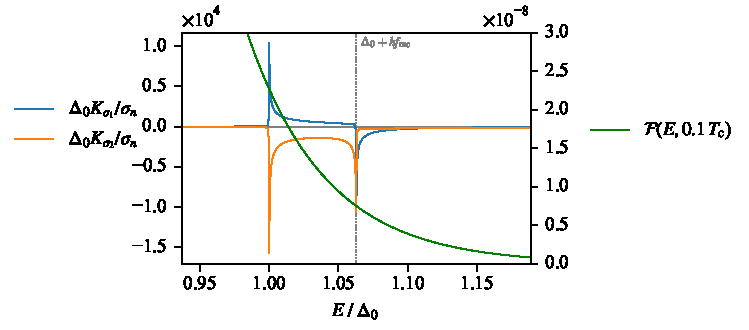
\includegraphics[width=\textwidth]{theory/responseqpoccupancy_conductivity_f_mc.pdf}
\caption
[The first-order response functions for the real and imaginary parts of the conductivity at $\freadout_\multichroic$.]
{The first-order response functions for the real and imaginary parts of the conductivity at $\freadout_\multichroic = \SI{3.0}{GHz}$ versus energy in units of the gap, and a thermal occupancy.
The left axis shows Equations~\ref{eqn:responseqpoccupancy_reconductivity} and~\ref{eqn:responseqpoccupancy_imconductivity} multiplied by constants to make them dimensionless.
For display, the density of states factors have been broadened using $\mitrovic / \gap_\zerotemp = 0.0002$.
The right axis shows a thermal occupancy at a typical KID operating temperature.
Figure~\ref{fig:responseqpoccupancy_conductivity_f_1p} shows the same quantities at a much lower frequency, where the peaks in the response functions are closer together.}
\label{fig:responseqpoccupancy_conductivity_f_mc}
\end{figure}

These expressions for $\responseqpoccupancy_{\reconductivity}$ and $\responseqpoccupancy_{\imconductivity}$ are plotted for two different frequencies in Figures~\ref{fig:responseqpoccupancy_conductivity_f_mc} and~\ref{fig:responseqpoccupancy_conductivity_f_1p}.
The absorption of readout photons by the quasiparticle system may decrease the occupancy at the gap and increase it at integer multiples of the readout photon energy.
While $\responseqpoccupancy_{\imconductivity}$ is negative for quasiparticles at all energies, $\responseqpoccupancy_{\reconductivity}$ is positive for frequencies near the gap but is negative for quasiparticles with energies higher than the gap plus one readout photon.
Shifting a quasiparticle from $\gap_\zerotemp$ to $\gap_\zerotemp + \planck \freadout$ will have a minor effect on $\imconductivity$, but will flip the sign of its effect on $\reconductivity$.
Thus, we expect the readout signal to have a larger effect on the dissipation in a resonator than on its resonance frequency.

To discuss perturbations around a steady-state situation in Section~\ref{sec:theory.response}, I use these response functions with the additional \textit{proportional-perturbation} assumption, namely, that perturbations $\delta\qpoccupancy$ to the occupancy are proportional to the steady-state occupancy $\ssqpoccupancy$.
If the perturbation varies in time, then $\delta\qpoccupancy(\energy, \time) / \ssqpoccupancy(\energy) = \epsilon(\time)$ for all energies $\energy$, where $\epsilon(\time) \ll 1$ (usually) is the fractional size of the perturbation.
This assumption is not necessarily true, especially for larger perturbations, but it greatly simplifies calculations because, as discussed in Section~\ref{sec:theory.qpnumber}, it allows us to write all perturbations in terms of perturbations to the quasiparticle number.

If
$C - C(0) = \braket{\responseqpoccupancy_C}{\qpoccupancy}$
is the shift in some quantity $C$ from the zero-temperature value $C(0)$ resulting from the occupancy $\ssqpoccupancy$,
and if
$\delta C(\time) = \braket{\responseqpoccupancy_C}{\delta\qpoccupancy(\time)}$
is the perturbation to the steady-state value resulting from a perturbation $\delta\qpoccupancy(\time)$ to $\ssqpoccupancy$,
we have
\begin{equation}
\epsilon(\time)
  =
  \frac{\delta\qpoccupancy(\energy, \time)}{\ssqpoccupancy(\energy)}
  =
  \frac{\braket{\responseqpoccupancy_C}{\delta\qpoccupancy(\time)}}
  {\braket{\responseqpoccupancy_C}{\ssqpoccupancy}}
  =
  \frac{\delta C(\time)}{C - C(0)}.
\end{equation}
That is, the fractional perturbations to all such quantities are equal.
Equivalently, the derivative of one first-order quantity with respect to another equals the ratio of the shifts from the zero temperature values:
\begin{equation}
\frac{\delta A(\time)}{\delta B(\time)}
  =
  \frac{\braket{\responseqpoccupancy_A}{\delta\qpoccupancy(\time)}}
  {\braket{\responseqpoccupancy_B}{\delta\qpoccupancy(\time)}}
  =
  \frac{\braket{\responseqpoccupancy_A}{\qpoccupancy}}
  {\braket{\responseqpoccupancy_B}{\qpoccupancy}}
  =
  \frac{A - A(0)}{B - B(0)},
\end{equation}
which is constant in time.
